\documentclass{article}
\usepackage{amsmath} % Для математических формул
\usepackage{enumitem} % Для настройки списков
\usepackage{tikz} % Для диаграмм Эйлера
\usepackage[utf8]{inputenc}
\usepackage[russian]{babel} % Для поддержки русского языка
\usepackage{array}
\usepackage{graphicx} % Для вставки фото


\title{Конспекты по ИПС}
\author{Минкин Даниэль}

\begin{document}

    \maketitle

    \tableofcontents

    \section{Введение}

        Мой ИПС посвящен построению скоринговой модели для предсказания потребительского дефолта.
        В рамках данного конспекта я собираю необходимую информацию из предоставленных куратором материалов

    \section{Риск}

        \begin{quote}
            \textbf{Риск} --- это влияние неопределенности на цели.
        \end{quote}

        \begin{itemize}
            \item Влияние - это отклонение от ожидаемого результата
            \item Цель - некий набор результатов (не обяз. с зад вероятностями)
            \item Неопределенность - это отсутствие информации о событии
        \end{itemize}

        \quad

        \begin{quote}

            \textbf{Источник риска} --- сущность, которая самостоятельно или
            в комбинации с другими обладает возможностью вызывать
            повышение риска, i.e повышает вероятность того, что неопределенность повлияет на цель
        \end{quote}

        \begin{quote}
            \textbf{Экспозиция} --- степень подверженности организации событию
        \end{quote}

        \begin{quote}
            \textbf{Стейкхолдер (i.e причастная сторона)} --- сущность подвергающаяся воздействию риска i.e берущая на себя риск
        \end{quote}

    \section{Риск-менеджмент}

        \subsection{Факторы, которые необходимо знать о риске}
            \begin{itemize}
                \item Что является источником риска?
                \item Рисковое событие
                \item Какие последствия из тех, что произойдут при реализации риска нас интересуют?
                \item Экспозицию риска
                \item Степень возможности наступления события, выраженная как вероятность
            \end{itemize}

       \subsection{Риски и убытки}


            Риск не связан с убытками, так как часть из них может быть достоверно определена и уже заложена при планировании

            \quad

            Убытки разделяются на два вида:

            \begin{itemize}
                \item \textbf{Ожидаемые} То, в чем мы уверены и заложили
                \item \textbf{Неожидаемые} Возможны, но не обязательны. Поэтому их необходимо оценить
            \end{itemize}


        \subsection{Что не входит в задачи риск-менеджмента?}

            \begin{itemize}
                \item Определение риска (это задачи аналитика или трейдера)
                \item Принятие решений
            \end{itemize}

            \begin{quote}
                \textbf{I.e риск менеджмент только просчитывает риски}
            \end{quote}

        \subsection{Суть риск-менеджмента}
            \begin{itemize}
                \item Риск не нужно минимизировать
                \item Риск-менеджмент определяет какие виды рисков нужно принимать, а какие нет
                \item Риск-менеджмент занимается неожиданными убытками
                \item Риск-менеджмент не предсказывает будущее, однако позволяет рассмотреть различные сценарии и дать им оценку
                \item Риск-менеджмент оценивает величину запасов
            \end{itemize}
    \section{Кредитный риск}
        \subsection{Особенности кредитного риска}
            \begin{itemize}
                \item Асимметрия: у нас ограниченные доходы, но существенные убытки
                \item Распределение с тяжелыми хвостами для доходности
                \item Распределение доходностей не является нормальным
                \item Более длительный горизонт планирования
                \item Меньше наблюдаемых данных
                \item Дефолты редки, поэтому мало past data
            \end{itemize}

        \subsection{Компоненты кредитного риска}
            \begin{itemize}
                \item \textbf{EAD} (Exposure at Default) - экспозиция при дефолте
                \item \textbf{PD} (Probability of Default) - вероятность дефолта
                \item \textbf{LGD} (Loss Given Default) - сумма, которую мы получаем при дефолте (убытки или возможно прибыли). Определяется как относительная величина, а не абсолютная
            \end{itemize}

            Все компоненты определяются как случайные процессы, т.е эти параметры могут изменятся со временем

            \begin{itemize}
                \item EAD - сумма платежных обязательств, должника (за вычетом обеспечения) на момент дефолта
                \item Recovery rate - доля риска, которая может быть взыскана в ходе процедуры банкротства

            \end{itemize}

            \begin{equation}
                LGD = (1 - recovRate)
            \end{equation}

            где $recovRate$ - recovery rate

            Следовательно, в случае дефолта потери составят:

            \begin{equation}
                Loss_{i} = EAD * LGD
            \end{equation}

            Общий loss скалывается из суммы loss - ов


            \begin{quote}
                \textbf{Риск концентрации} --- ситуация когда индивидуальные потери внутри портфеля сильно коррелированы
            \end{quote}

        \subsection{Эмпирические данные о распредлении потерь портфеля}
            \begin{itemize}
                \item Асимметрия слева
                \item Тяжелые хвосты
                \item PD и EAD коррелированны
                \item LGD и EAD не коррелированны
                \item PD и LGD коррелированны
                \item Корреляции случайны
            \end{itemize}

        \subsection{Мат. ожидание потерь}

            \begin{equation}
                \mathrm{E}[loss_{i}] = PD_{i} * EAD_{i} * LGD_{i}
            \end{equation}

            При условии, что $EAD_{i}$ и $LGD_{i}$ независимы
            \begin{quote}
                \textbf{Неожидаемый убыток} --– это разница между фактическим убытком и ожидаемым убытком
            \end{quote}

        \subsection{Right и Wrong way риски}

            \begin{quote}
                \textbf{Wrong-way риск} --- ситуация, при которой экспозиция контрагента положительно коррелирует с вероятностью дефолта этого контрагента

            \end{quote}

            I.е вероятность дефолта падает, но сумма, которую мы должны от него получить снижается

            \begin{quote}
                \textbf{Right-way риск} -- ситуация, при которой $EAD$ и $PD$ коррелируют положительно
            \end{quote}
    \section{ROC - кривая}
        \begin{quote}
            \textbf{ROC} (Receiver Operating Characteristic curve) --- кривая операционной характеристики получателя,
            кривая на которой по оси Y расположен \textbf{true positive rate} или
            \textbf{чувствительность модели}, а по оси X \textbf{false positive rate} или \textbf{специфичность модели}
        \end{quote}

        Предполагается, что у нас есть гиперпараметр, меняя который можно регулировать кол-во TP и FP.
        Данный параметр часто называется \textbf{точкой отсечения} (\textbf{cut-off value}) --- некая величина
        $p_{limit}$ такая, что если $p_{predicted} > p_{limit}$ то клиент считается дефолтным. Получается регулируя
        данный параметр мы можем менять оценку кол-ва дефолтных клиентов.

        \begin{center}
            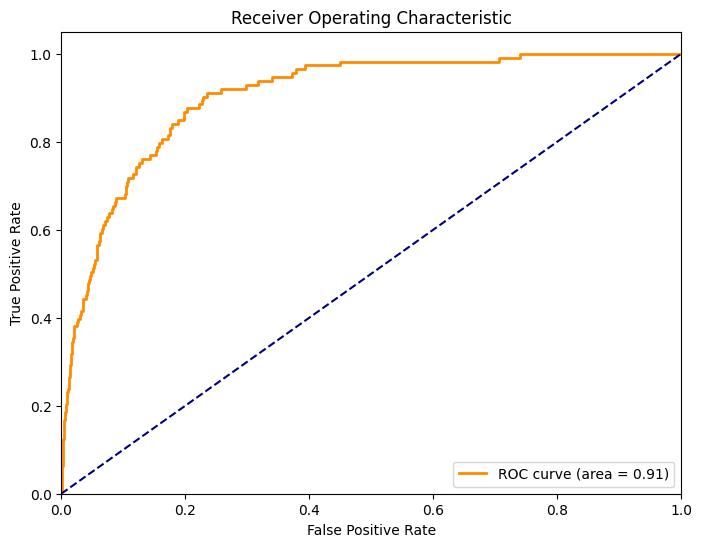
\includegraphics[width=0.5\textwidth]{photos/roc.png}
        \end{center}



        \subsection{TPR и FPR}
            \begin{table}[h] % [h] для размещения таблицы "здесь"
                \centering % Центрирование таблицы
                \caption{Исходы предсказания} % Заголовок таблицы
                \begin{tabular}{|c|c|c|}
                    \hline
                    & \textbf{Предсказано: Да} & \textbf{Предсказано: Нет} \\ \hline
                    \textbf{Фактически: Да} & True Positive (TP) & False Negative (FN) \\ \hline
                    \textbf{Фактически: Нет} & False Positive (FP) & True Negative (TN) \\ \hline
                \end{tabular}
            \end{table}
    
            \begin{equation}
                TPR = \dfrac{TP}{TP + FN}
            \end{equation}
            Intuition: Получается мы берем, все случаи когда произошел дефолт и смотрим, какую
            долю произошедших дефолтов мы предсказали
    
            \begin{equation}
                FPR = \dfrac{FP}{FP + TN}
            \end{equation}
            Intuition: В этот раз мы смотрим на все случаи, когда дефолт не произошел и смотрим, долю ошибок нашей
            модели - когда мы сказали, что дефолт будет, но его не было
    
        \subsection{Precision и Recall}
            Precision и Recall - очень похожие метрики

            \begin{equation}
                Precision = \dfrac{TP}{TP + FP}
            \end{equation}
            В этот раз, мы рассматриваем все случаи, когда мы предсказали ``Да`` и оцениваем какая доля из этих предсказаний, оказалась правильной

            \begin{equation}
                Recall = TPR
            \end{equation}
    
        \subsection{Accuracy}
            Accuracy используется для оценки общего качества модели,
            мы рассматриваем долю всех правильных ответов модели.


            \begin{equation}
                Accuracy = \dfrac{TP + TN}{TP + TN + FP + FN}
            \end{equation}

    \section{ROC AUC}
        ROC AUC расшифровывается как ROC area under curve. Нам важна не самая кривая а ее форма. Поэтому для сравнитаельной
        оценки качества моделей, часто применяется сравнение площадей под ними. Легко заметить, что
        идеальная модель, будет иметь площадь под графиком равную единице, т.е кривая будет проходить по верхней границе
        $y = 1$ при любом $x$. (I.e мы будем предсказывать все случившиеся дефолты на 100\% при этом во всех случаях, когда дефолта
        не было мы так и сказали). Также можно легко заметить, что если площадь под кривой менее 0.5, то наша модель хуже случайного
        классификатора, так как он представляет собой прямую $y = x$ (точка такой модели зависит от cut-off value)

        \quad

        Таким образом, с помощью AUC мы можем сравнивать качество моделей, однако данный показатель имеет мало смысла в абсолютном значении

        \quad

        На практике все определяется конкретными требованиями к модели, так модель с меньшим AUC может подходить больше за счет того, что она проходит через определенные точки
























\end{document}